\section{Control Flow Graph (CFG) dan Peephole Optimization}

Setelah optimasi level blok (\textit{local}), kompilator mulai memandang program secara keseluruhan melalui struktur graf dan jendela instruksi kecil.

\subsection{1. Membangun Control Flow Graph yang Kompleks}
CFG memetakan alur eksekusi antar blok. Terdapat dua jenis arah panah (\textit{edges}):
\begin{itemize}
    \item \textbf{Fall-through}: Dari $B_1$ ke $B_2$ jika $B_2$ terletak tepat di bawah $B_1$ dan $B_1$ tidak berakhir dengan lompatan mutlak.
    \item \textbf{Jump}: Dari $B_1$ ke $B_2$ jika instruksi terakhir $B_1$ adalah lompatan ke label di awal $B_2$.
\end{itemize}

\subsection{2. Peephole Optimization}
\compiler{Peephole Optimization} adalah teknik machine-dependent yang menganalisis "jendela" kecil berisi 2-3 instruksi target (\textit{assembly/machine code}) untuk mencari pola yang bisa dipercepat.

Teknik umum dalam Peephole:
\begin{enumerate}
    \item \textbf{Redundant Load/Store Elimination}: Menghapus instruksi \texttt{STORE} variabel jika variabel tersebut langsung di-\texttt{LOAD} kembali tanpa perubahan.
    \item \textbf{Unreachable Code}: Menghapus instruksi yang muncul setelah \texttt{goto} atau \texttt{return} mutlak yang tidak memiliki label.
    \item \textbf{Flow of Control Optimization}: Mengganti \texttt{goto L1} di mana \texttt{L1} berisi \texttt{goto L2} menjadi langsung \texttt{goto L2}.
    \item \textbf{Algebraic Hints}: Mengganti operasi matematika dengan instruksi mesin yang lebih efisien (misal: \texttt{INC} alih-alih \texttt{ADD 1}).
\end{enumerate}

\begin{figure}[!htbp]
    \centering
    \adjustbox{max width=0.8\textwidth,center}{%
    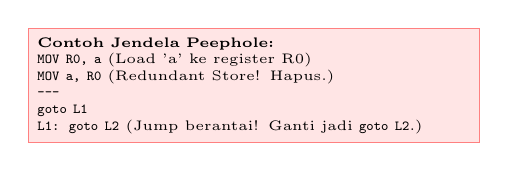
\begin{tikzpicture}[
        rect/.style={rectangle, draw=red!50, fill=red!10, text width=5.5cm, font=\tiny}
    ]
    \node[rect] (peephole) {
        \textbf{Contoh Jendela Peephole:}\\
        \texttt{MOV R0, a}  (Load 'a' ke register R0)\\
        \texttt{MOV a, R0}  (Redundant Store! Hapus.)\\
        \texttt{---}\\
        \texttt{goto L1}\\
        \texttt{L1: goto L2} (Jump berantai! Ganti jadi \texttt{goto L2}.)
    };
    \end{tikzpicture}%
    }
    \caption{Mekanisme Jendela (Peephole) pada Level Kode Mesin}
\end{figure}

\subsection{Menuju Optimasi Global}
Optimasi lokal dan peephole memberikan dasar yang kuat. Langkah berikutnya adalah \textit{Data Flow Analysis} (Chapter 9) yang menggunakan CFG untuk melacak nilai variabel di seluruh fungsi, memungkinkan optimasi seperti \textit{Global Dead Code Elimination}.
    
